% file: math/full-binary-tree-LR.tex

\documentclass{standalone}
\usepackage{tikz}
\usepackage{tikz-qtree}

\usetikzlibrary{backgrounds, fit, shapes, calc}

\begin{document}

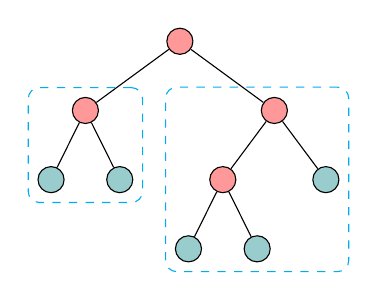
\begin{tikzpicture}[level distance = 25pt, sibling distance = 15pt,
  edge from parent/.style= {
      draw, edge from parent path = {(\tikzparentnode) -- (\tikzchildnode)}}]
  \tikzset{every tree node/.style = {align = center, circle, draw, fill = red!40},
      leaf/.style = {fill = teal!40}}

	  \Tree [.{} 
	          [.\node[](l){}; 
	  		[.\node[leaf](l1){}; ]
		        [.\node[leaf](l2){}; ]
                  ]
		  [.\node[](r){};
		    [.\node[](rl){};
		      [.\node[leaf](l3){}; ] 
		      [.\node[leaf](l4){}; ]
		    ] 
		    [.\node[leaf](l5){}; ]
		  ] 
	  ]

  \coordinate (rr) at ($(r)-(0, .7)$);

  \node () [draw, dashed, cyan, rounded corners, fit = (l) (l1) (l2)] {};
  \node () [draw, dashed, cyan, rounded corners, fit = (rl) (rr) (l3) (l4) (l5)] {};
\end{tikzpicture}
\end{document}
